\documentclass{beamer} %
\usetheme{Dresden}
\usecolortheme{beaver}
\usepackage[ngerman, english]{babel}
\usepackage[utf8x]{inputenc}
\usefonttheme{professionalfonts}
\usepackage{times}
\usepackage{tikz}
\usepackage{amsmath}
\usepackage{tabulary}
\usepackage{pgfgantt}
\usepackage{verbatim}
\usetikzlibrary{arrows,shapes}
\usepackage{adjustbox}
\usepackage{soul}
\usepackage{listings}
\usepackage{adjustbox}
\setbeamertemplate{itemize item}{\color{red}$\blacksquare$}
\usepackage{hyperref}
\usepackage{multicol}
\usepackage{animate}
\title{avance1}
\setbeameroption{}

\title{Architektur \\für skalierbare Webanwendungen}
\institute[]{Hochschule für angewandte Wissenschaften München\\Fakultät für Informatik und Mathematik}
\date[07.06.2017]{07.~Juni 2017}
%\titlegraphic{
\includegraphics[height=2cm]{img/HMLogoFK07.png}}

\author{Vladislav Faerman}
%\date{\today}

\begin{document}
\tikzstyle{every picture}+=[remember picture]
\lstset{language=R}   
\everymath{\displaystyle}

\AtBeginSection[]{ 


\begin{frame}
 \begin{multicols}{2}
	\frametitle{Agenda}
	\tableofcontents[currentsection,subsubsectionstyle=shaded]
	 \end{multicols}
\end{frame}
}

\begin{frame}[plain]
	\titlepage
\end{frame}



\section[Einleitung]{Einleitung}
\subsection{Motivation}
\begin{frame}
%\frametitle{Motivation und Ziel}
Projekte, die rapide populär werden und ein exponentielles Anwenderwachstum erleben, sind sehr oft nicht im Stande mit rasant steigender Anzahl von Anfragen und großen Datenmengen effizient umzugehen.\newline\newline

Für dieses ernsthaftes Problem kommen zwei wichtige Punkte in Betracht:
\begin{itemize}
\item Skalierbarkeit und 
\item Wartbarkeit
\end{itemize}
%Architektur für Webanwendungen aufstellen, die die Entwicklung von skalierbaren, wartungs- und erweiterungsfähigen Webanwendungen ermöglicht.
\note{test}
\end{frame}





\section[Theorie]{Theorie}
\subsection{Skalierbarkeit}

\begin{frame}
\frametitle{Skalierbarkeit}

Die Fähigkeit eines Systems, aufgrund der wachsenden Anforderungen, entweder die Leistung der vorhandenen Ressourcen zu verbessern oder zusätzlich die neuen Ressourcen hinzufügen.\newline\newline

Bei der Skalierbarkeit sind zwei Arten zu unterscheiden, eine \textit{vertikale} und eine \textit{horizontale} Skalierbarkeit.
\end{frame}


\begin{frame}
\frametitle{Vertikale Skalierbarkeit}

Anstreben einer qualitativen Steigerung der Leistungsfähigkeit der bereits eingesetzten Ressourcen.

\end{frame}

\begin{frame}
\frametitle{Horizontale Skalierbarkeit}

Im Gegensatz zur vertikalen Skalierbarkeit wird bei der horizontalen Skalierbarkeit die Last auf zusätzliche Rechner verteilt.

\end{frame}

%\begin{frame}
%\frametitle{ACID-Prinzip}
%
%\begin{itemize}
%\item  \textbf{A}tomicity (Atomarität)
%\begin{itemize}
%\item die Transaktion wird entweder ganz oder gar nicht ausgeführt
%\end{itemize}
%\item  \textbf{C}onsistency (Konsistenz)
%\begin{itemize}
%\item vor und auch nach dem Ablauf einer Transaktion werden die Integrität und Plausibilität der Datenbestände gewährleistet
%\end{itemize}
%\item  \textbf{I}solation (Isolation)
%\begin{itemize}
%\item um unerwünschte Nebenwirkungen zu vermeiden, werden die Transaktionen gekapselt
%\end{itemize}
%\item  \textbf{D}urability (Dauerhaftigkeit)
%\begin{itemize}
%\item gewährleistet nach einer erfolgreichen Transaktion die Persistenz aller Datenänderungen 
%\end{itemize}
%
%\end{itemize}
%
%\end{frame}




%\begin{frame}
%\frametitle{ACID-Prinzip: Problem in verteilten Datenbanken}
%
%In verteilten Datenbanken kommt es zu Problemen, wenn alle ACID-Eigenschaften erfüllt werden sollen.
%
%%Diese Probleme wurden in dem CAP-Theorem von Brewer formuliert. Im Umfeld der NoSQL-Datenbanken wird daher häufig das BASE-Prinzip (Basically Available, Soft state, Eventual consistency) verfolgt.
%
%\end{frame}




\begin{frame}
\frametitle{Das CAP-Prinzip}

Im Jahr 2000 präsentierte Eric A. Brewer das CAP-Theorem - ein Ergebnis seiner Forschungen zu verteilten Systemen:\newline
\begin{itemize}
\item  \textbf{C}onsistency (Konsistenz)
\begin{itemize}
\item Korrektheit der in der Datenbank gespeicherten Daten, auch in allen replizierenden Knoten in einem Cluster
\end{itemize}
\item  \textbf{A}vailability (Hochverfügbarkeit)
\begin{itemize}
\item Alle Anfragen an das System werden mit akzeptabler Reaktionszeit stets beantwortet 
\end{itemize}
\item  \textbf{P}artition Tolerance (Partitionstoleranz) 
\begin{itemize}
\item Die Ausfalltoleranz eines Knotens bzw. eines Servers aus einem Cluster
\end{itemize}

\end{itemize}

\end{frame}

\begin{frame}
\frametitle{Das CAP-Prinzip}
\begin{center}
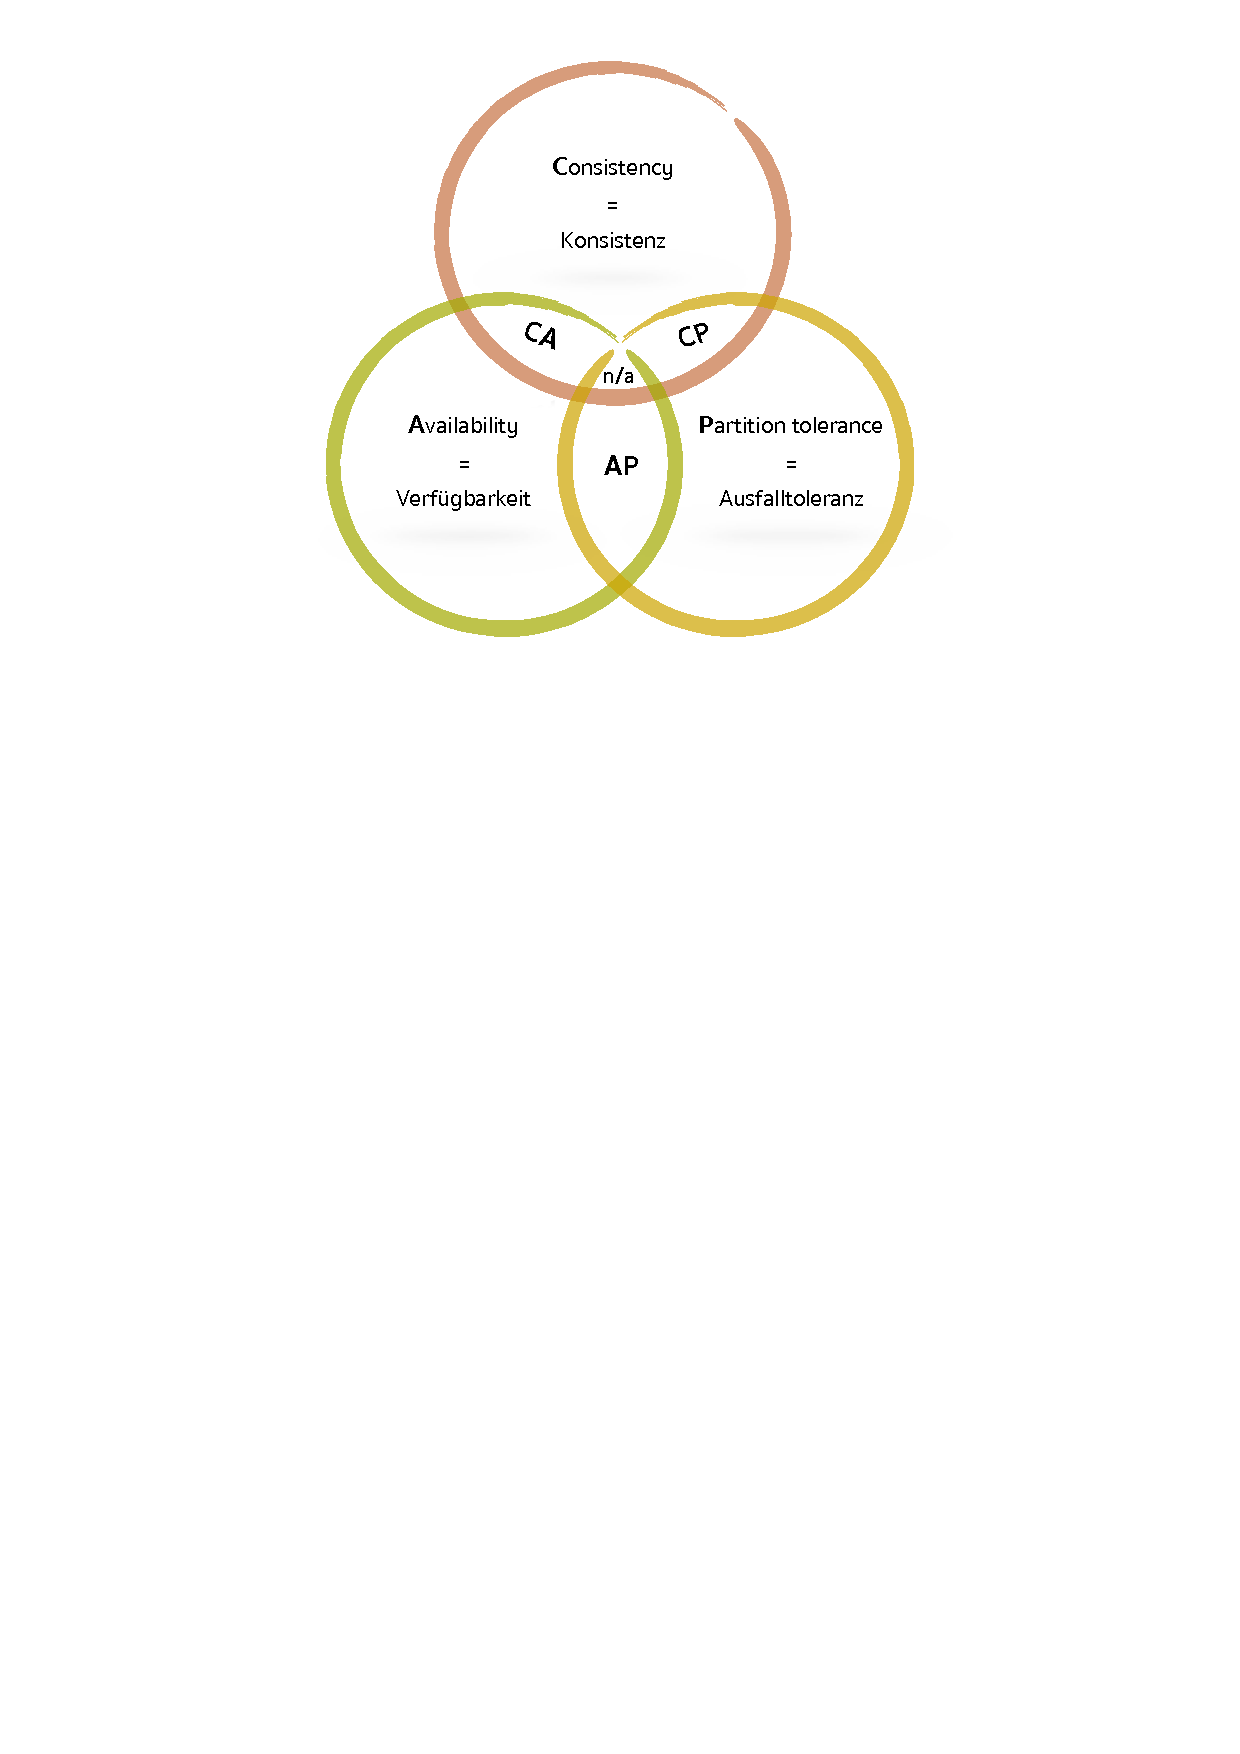
\includegraphics[trim = 0mm 189mm 0mm 9mm, clip, width=0.9\textwidth]{img/myPictureForCAP}
\end{center}
Die drei Anforderungen sind laut Brewer gleichzeitig nicht zu erfüllen.
\end{frame}


\begin{frame}
\frametitle{Das CAP-Prinzip}
Die Anforderungen in Paaren klassifizieren bestimmte Datenbanktechnologien.\newline
\begin{itemize}
\item  \textbf{CA} (\textbf{C}onsistency und \textbf{A}vailability)
\begin{itemize}
\item für die klassischen relationalen Datenbankmanagementsysteme (RDBMS)\newline
\end{itemize}

\item  \textbf{CP} (\textbf{C}onsistency und \textbf{P}artition tolerance)
\begin{itemize}
\item z. B. für Banking-Anwendungen\newline
\end{itemize}

\item  \textbf{AP} (\textbf{A}vailability und \textbf{P}artition tolerance)
\begin{itemize}
\item die Social-Media-Sites wie Twitter oder Facebook 
\end{itemize}

\end{itemize}

\end{frame}

%\begin{frame}
%\frametitle{Das BASE-Prinzip}
%
%Folgendes Prinzip beschreibt eine Alternative zu den strengen ACID-Kriterien und wird im Umfeld der NoSQL-Datenbanken verfolgt: \newline
%\begin{itemize}
%\item \textbf{B}asically \textbf{A}vailable
%\item \textbf{S}oft State
%\item \textbf{E}ventually Consistent \newline
%\end{itemize}
%
%Bei den Systemen, die nach dem BASE-Prinzip gestaltet sind, wird bewusst in Kauf genommen, dass die Daten nach Schreiboperationen eine absehbare Zeit inkonsistent sein können.
%
%\end{frame}

\subsection{Wartbarkeit}
\begin{frame}
\frametitle{Die SOLID-Prinzipien}

Fünf Prinzipien des objektorientierten Designs:\newline
\begin{itemize}
\item \textbf{S}ingle responsibility principle
\item \textbf{O}pen/closed principle
\item \textbf{L}iskov substitution principle
\item \textbf{I}nterface-segregation principle
\item \textbf{D}ependency inversion principle \newline
\end{itemize}

Bei korrekter Anwendung dieser Prinzipien erfolgt eine höhere Wartbarkeit am Softwareprodukt.

\end{frame}



%\begin{frame}
%\frametitle{\textbf{S}ingle responsibility principle (SRP)}
%Für die Änderung einer Klasse kann nur einen Grund geben.
%\end{frame}
%
%\begin{frame}
%\frametitle{\textbf{O}pen/closed principle (OCP)}
%Die Klassen/Module sollen für die Erweiterung offen sein, die bestehenden Klassen sollen jedoch nicht geändert werden.
%\end{frame}
%
%\begin{frame}
%\frametitle{\textbf{L}iskov substitution principle (LSP)}
%Die Subklassen dürfen das Verhalten der Elternklassen nicht ändern. Der Code, der auf bestehenden Funktionen der Elternklassen aufgebaut ist, muss auch mit Subklassen fehlerfrei funktionieren.
%\end{frame}
%
%\begin{frame}
%\frametitle{\textbf{I}nterface-segregation principle (ISP)}
%Die Interfaces sollen so klein wie möglich sein und nur einzelne Funktionen abdecken.
%\end{frame}
%
%\begin{frame}
%\frametitle{\textbf{D}ependency inversion principle (DIP)}
%Die Abhängigkeiten zwischen Modulen sollen über Abstraktionen (Interfaces) gekoppelt werden. Ein Modul soll eine direkte Abhängigkeit zu den anderen Modulen vermeiden, die Abhängigkeiten werden zu den Interfaces definiert.
%\end{frame}

\begin{frame}
\frametitle{Dependency Injection (DI)}
Dependency Injection ist der nächste Schritt nach Dependency Inversion.

\begin{itemize}
\item die Klassen haben die Abhängigkeiten nur zu den Interfaces
\item konkrete Implementierungen werden durch die externe Komponente zur Laufzeit eingefügt (injected).

\item \textbf{Ziel:} Anwendungsobjekte voneinander entkoppelt zu halten: \textbf{lose Kopplung}.
\end{itemize}
Diese ermöglicht dem Entwickler die Konzentration auf die Entwicklung einzelner Komponenten unabhängig voneinander.
\end{frame}

%\begin{frame}
%\frametitle{Dependency Injection (DI) und Mock-Objekte}
%bla
%\end{frame}

\addtocontents{toc}{\newpage} 

\section[Architektur]{Architektur}
\subsection[Architektur]{Konzept}

\begin{frame}
\frametitle{Typische Architektur einer Webanwendung}
\begin{center}
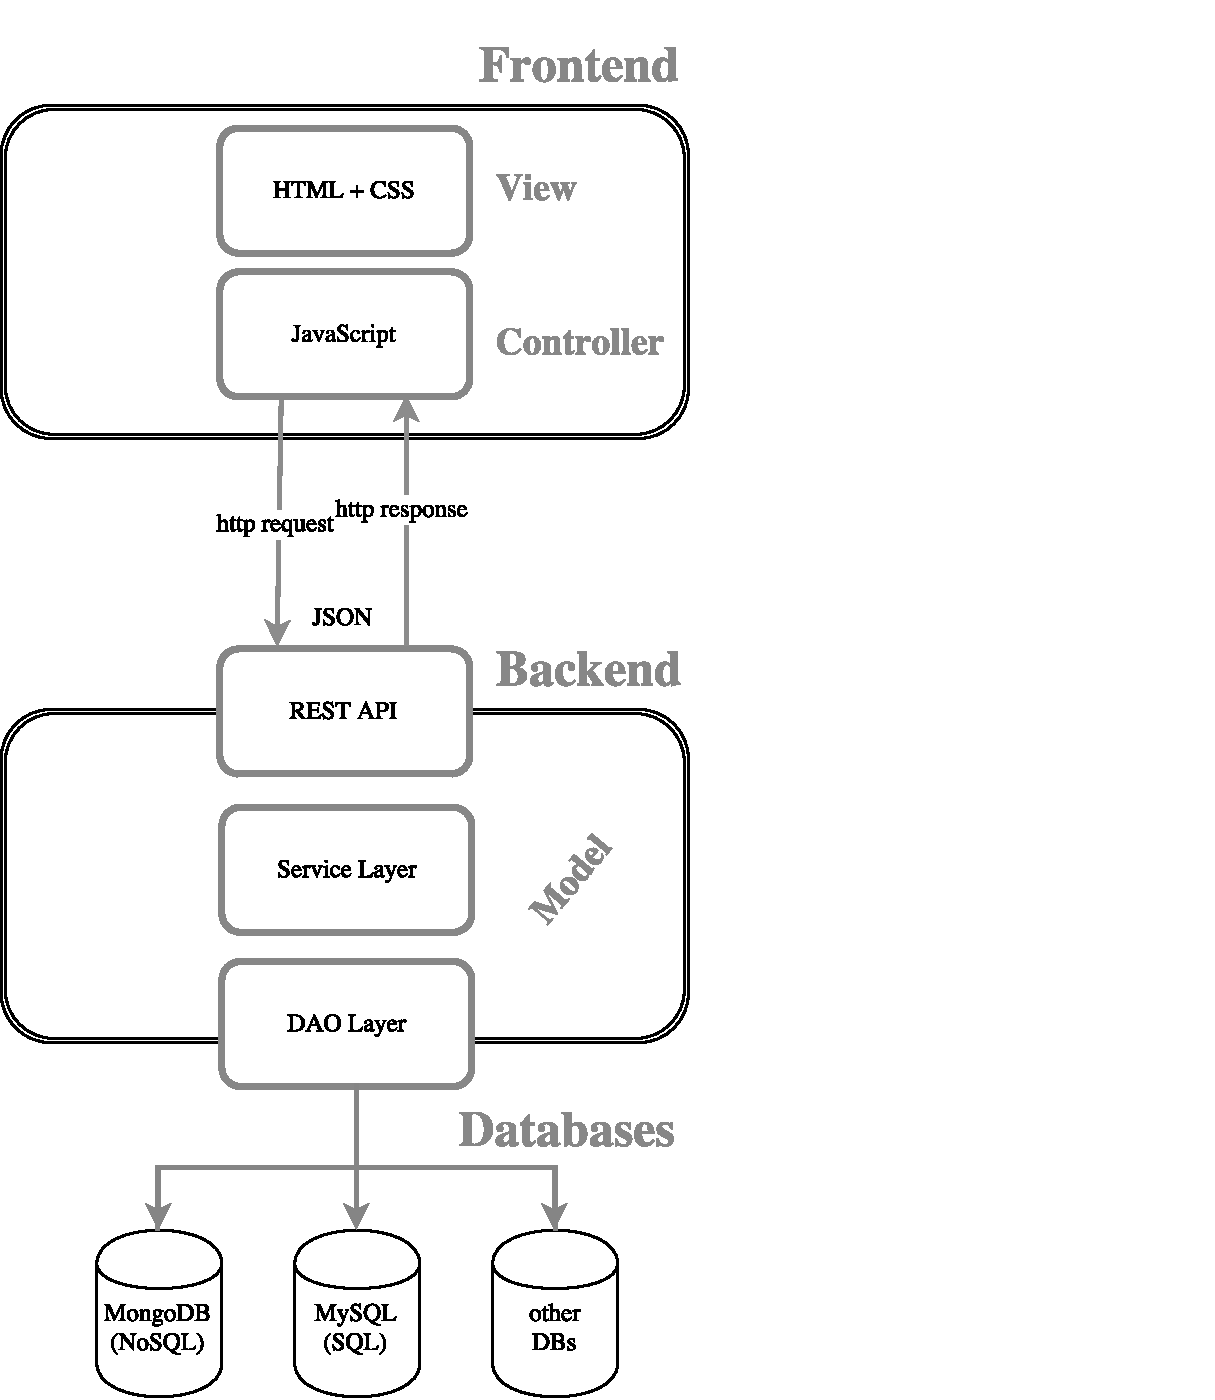
\includegraphics[trim = 0mm 0mm 0mm 5mm, clip, width=0.28\textwidth]{img/architectureMyAppWithoutFrameworks}
\end{center}
\end{frame}

\begin{frame}
\frametitle{Konzept}
\begin{center}
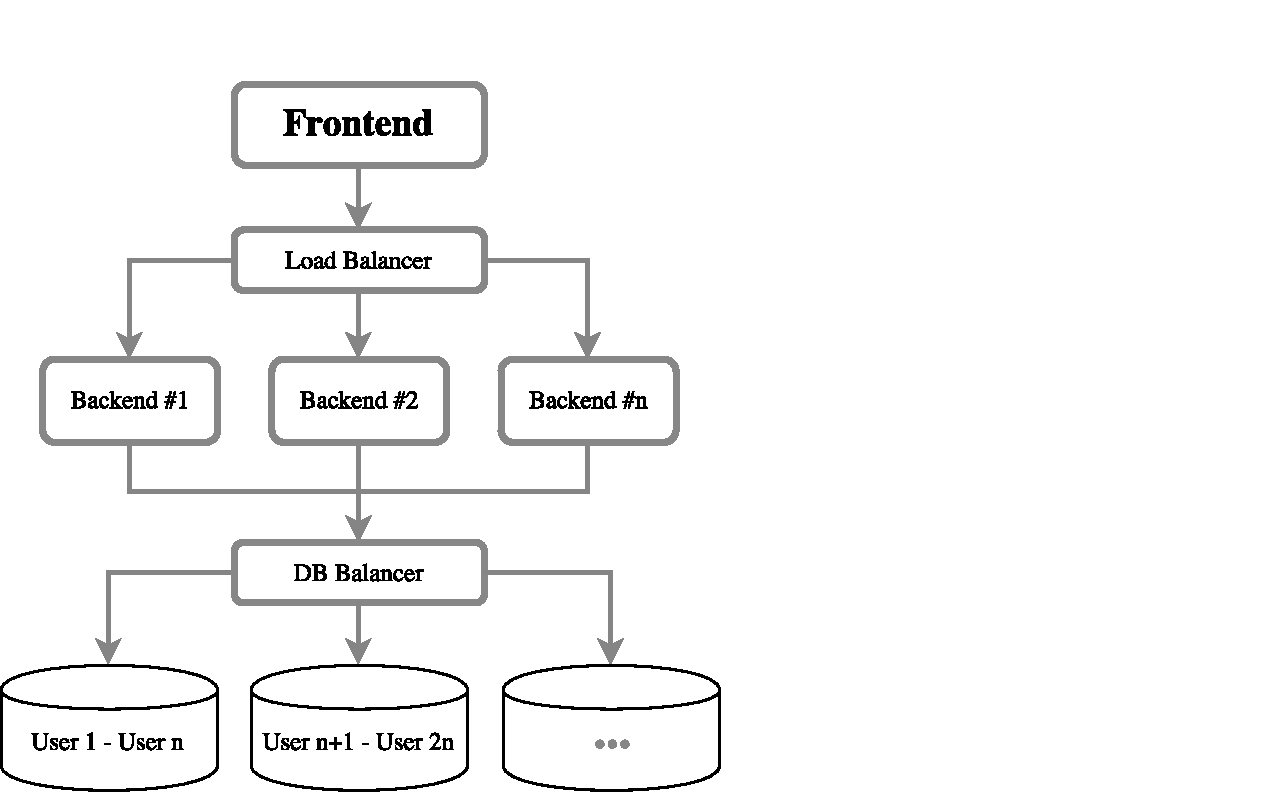
\includegraphics[trim = 0mm 0mm 0mm 0mm, clip, width=0.50\textwidth]{img/ueberblickArchitektur}
\end{center}
\end{frame}

\begin{frame}
\frametitle{Umsetzbarkeit}
\begin{center}
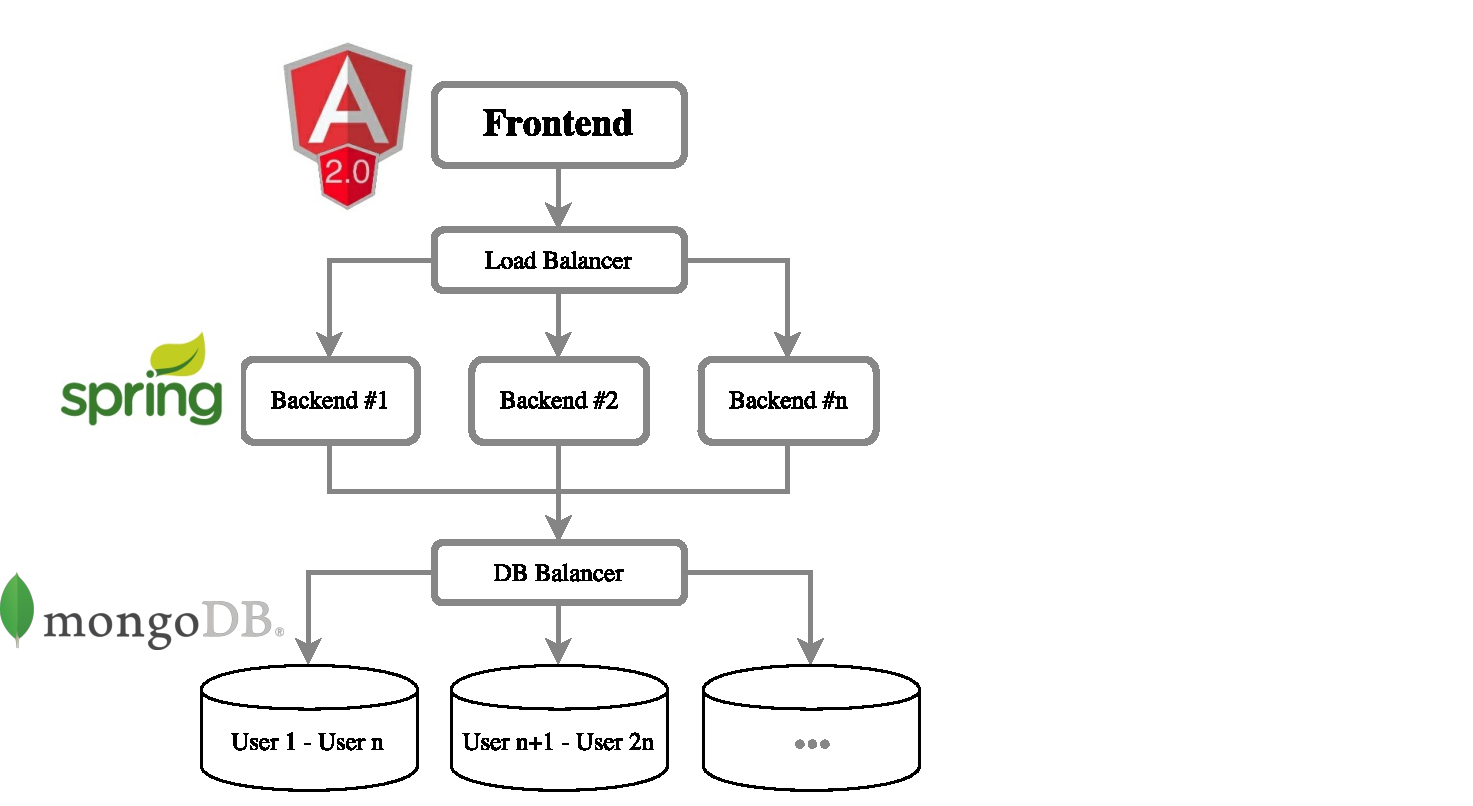
\includegraphics[trim = 0mm 0mm 0mm 0mm, clip, width=0.60\textwidth]{img/frameworks}
\end{center}
\end{frame}



%\begin{frame}
%\frametitle{MVC-Pattern}
%\textbf{MVC}  ist ein Prinzip der modernen Programmierung und ist nach wie vor das wichtigste und verbreitetste Muster für die Architektur von GUI-Anwendungen.\newline
%
%\textbf{Ziel:} die Geschäftslogik einer Anwendung von der Benutzerschnittstelle trennen, was eine spätere Änderung oder Erweiterung erleichtert und eine Wiederverwendbarkeit und Austauschbarkeit einzelner Komponenten ermöglicht.
%\end{frame}
%
%\begin{frame}
%\frametitle{Workflow zum MVC-Konzept}
%
%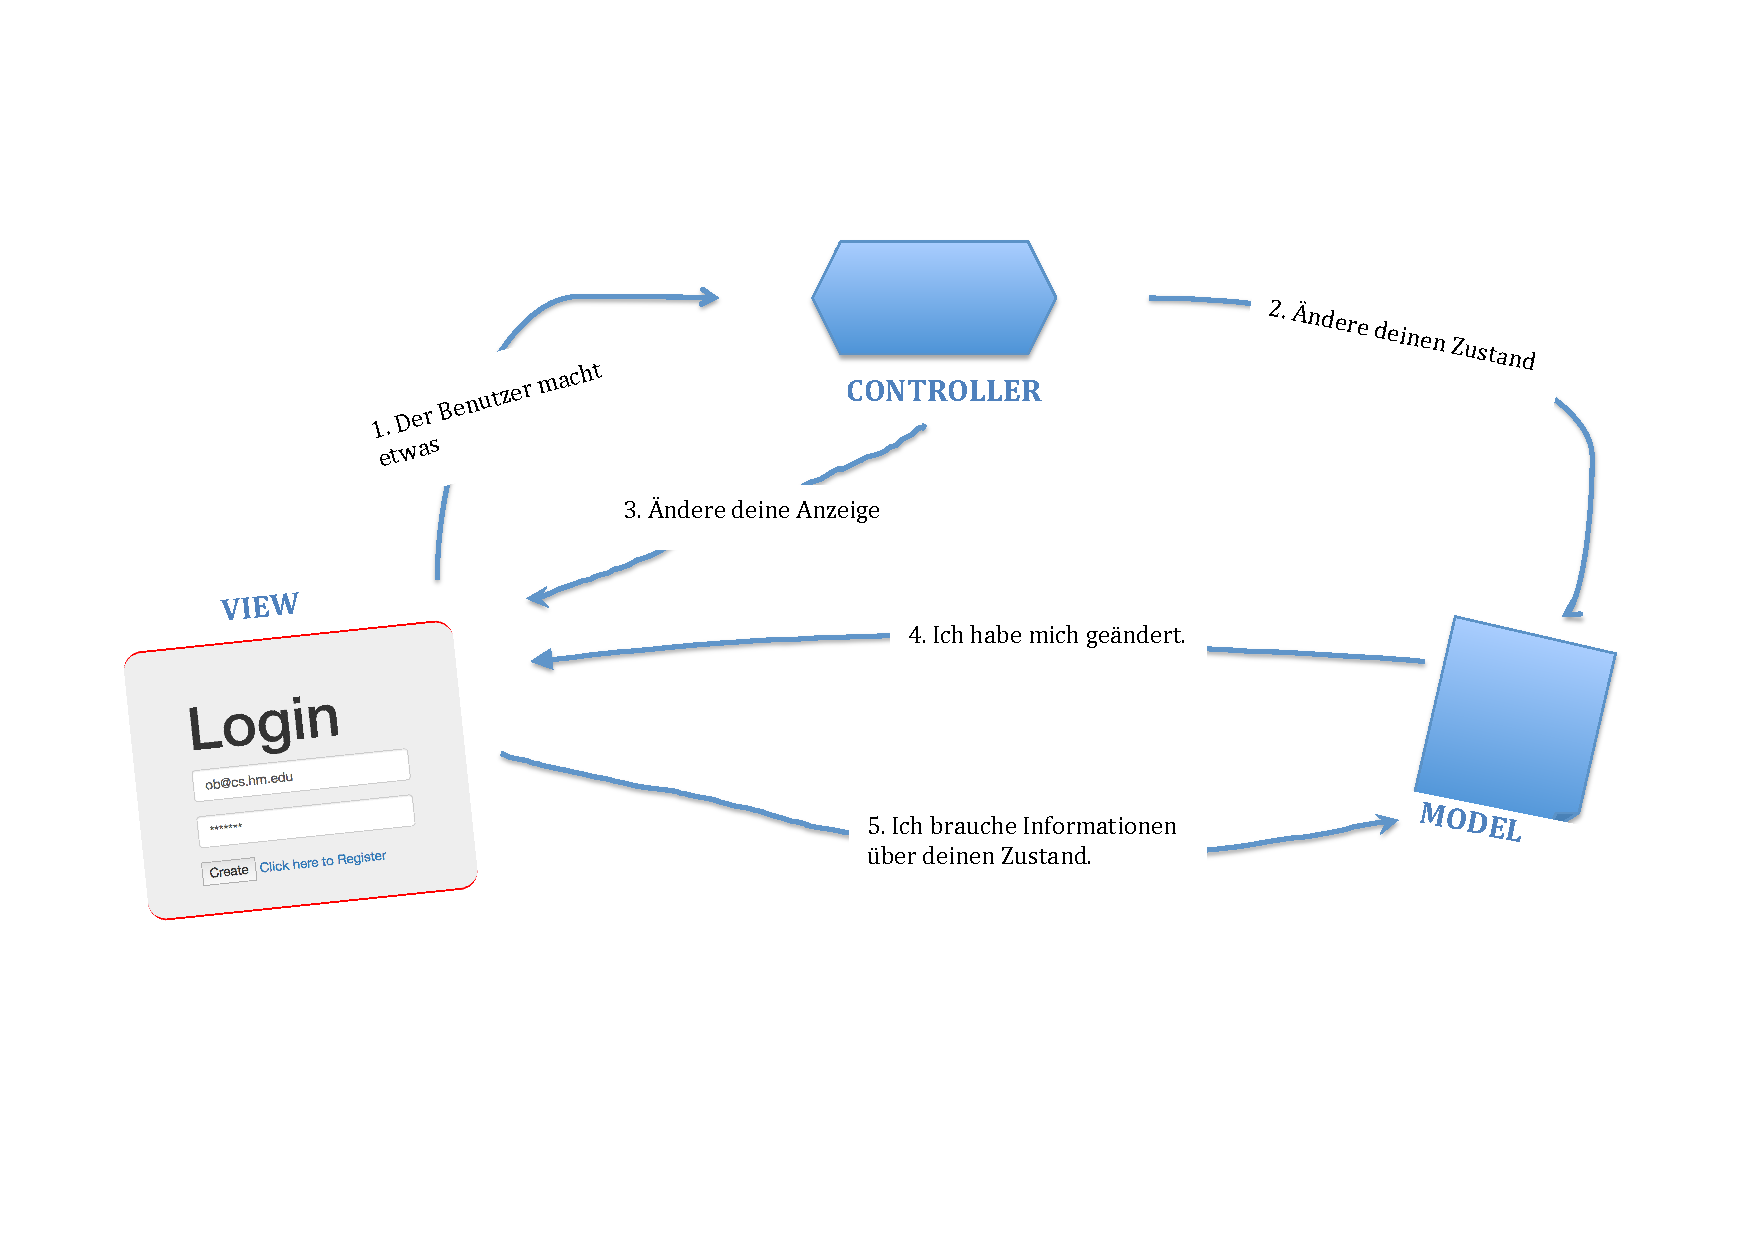
\includegraphics[trim = 0mm 20mm 0mm 30mm, clip, width=1.0\textwidth]{img/mvcAndOP}
%\end{frame}
%
%\begin{frame}
%\frametitle{Observer Pattern}
%\begin{center}
%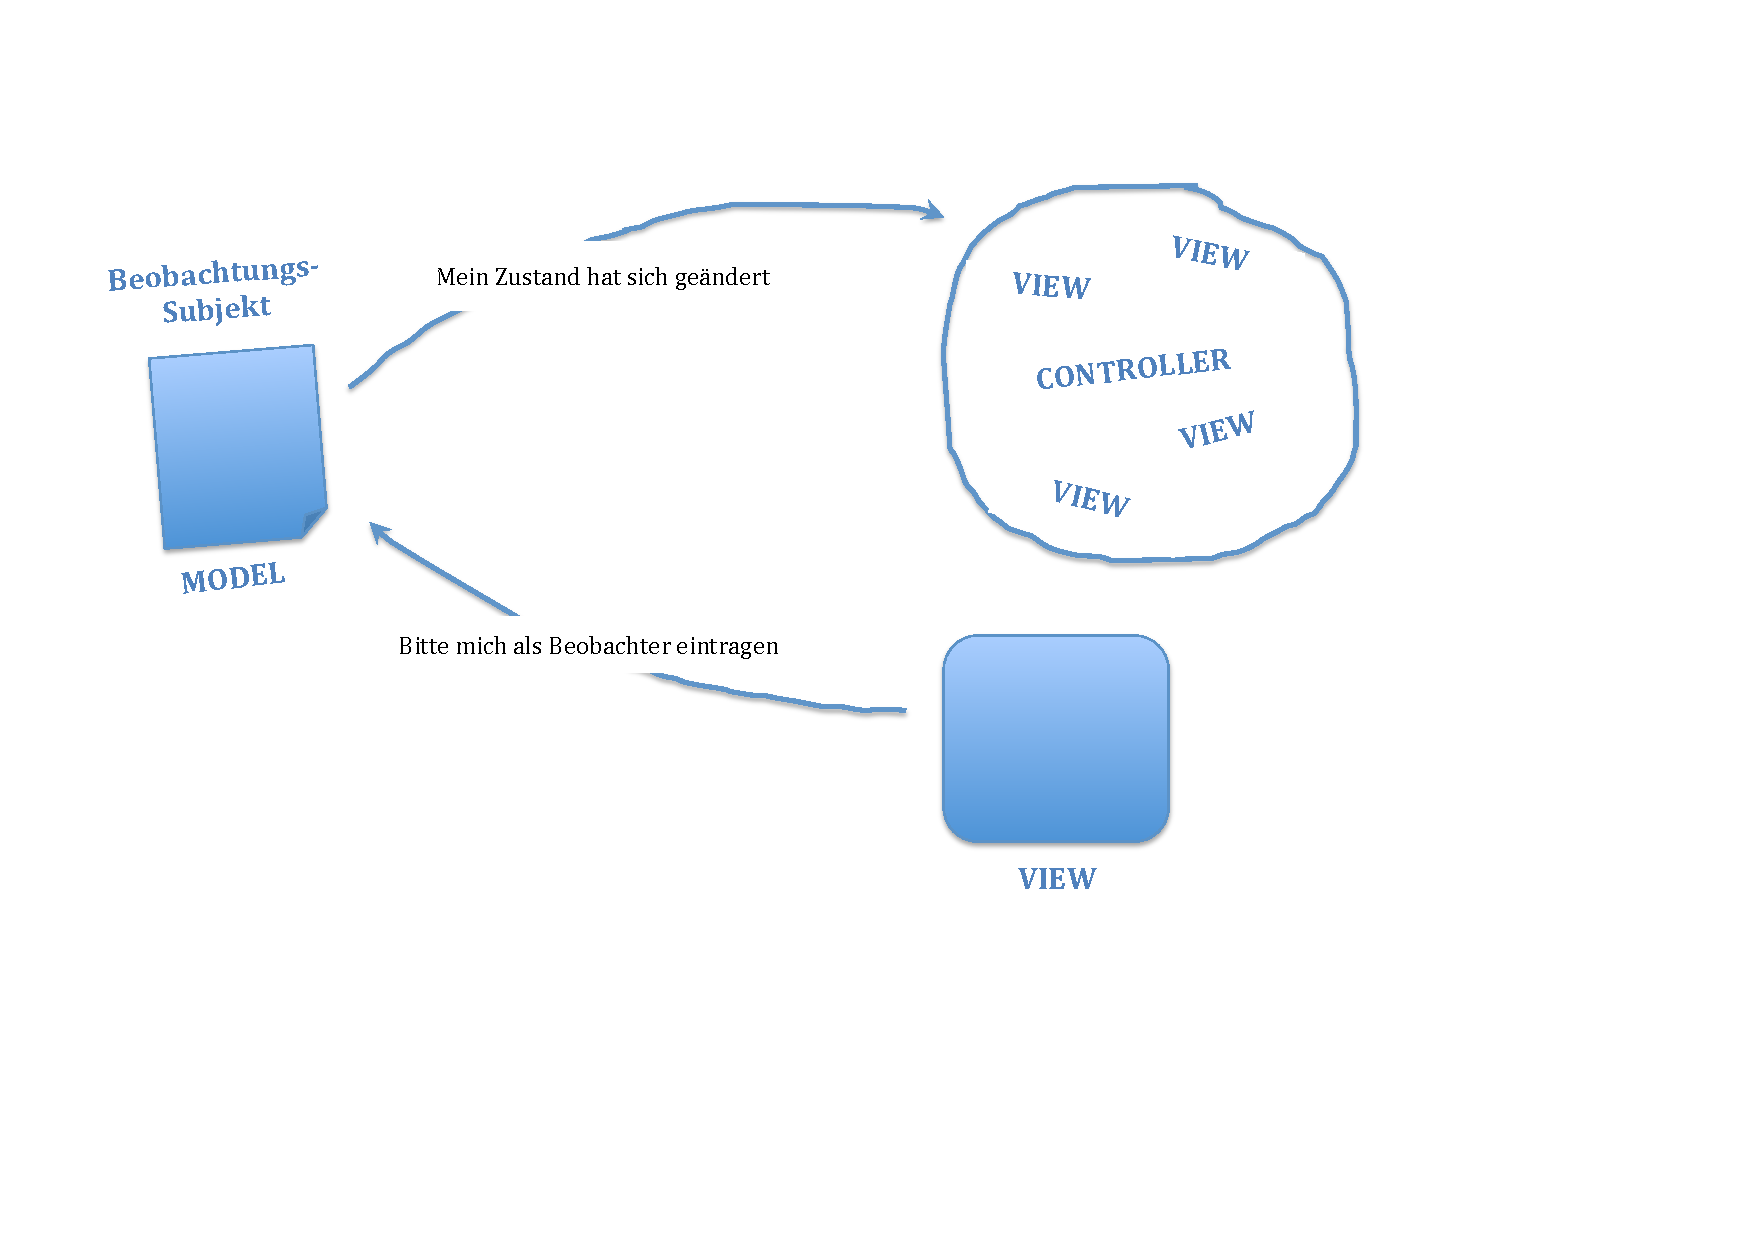
\includegraphics[trim = 0mm 0mm 0mm 0mm, clip, width=0.9\textwidth]{img/observer}
%\end{center}
%\end{frame}






\section{Relevante Technologien}
\begin{frame}
\frametitle{NoSQL-Datenbanken}
\textbf{NoSQL} erlaubt eine unstrukturierte Haltung von Daten.\newline\newline
Mögliche \textbf{NoSQL}-Kategorien:

\begin{itemize}

\item Key-Value-Datenbank
\item spaltenorientierte Datenbank
\item Graphen-Datenbank
\item dokumentenorientierte Datenbank

\end{itemize}
\end{frame}


\subsubsection*{MongoDB}
\begin{frame}
\frametitle{MongoDB}
\textbf{MongoDB} ist eine von vielen NoSQL-Datenbanken, die als eine schemalose, dokumentenorientierte Open-Source-Datenbank bekannt ist. \newline

Wichtige Konzepte sind \textbf{Ausfallsicherheit} und \textbf{horizontale Skalierung}.
\end{frame}

\begin{frame}
\frametitle{MongoDB: Replikation (Replication)}

\begin{center}
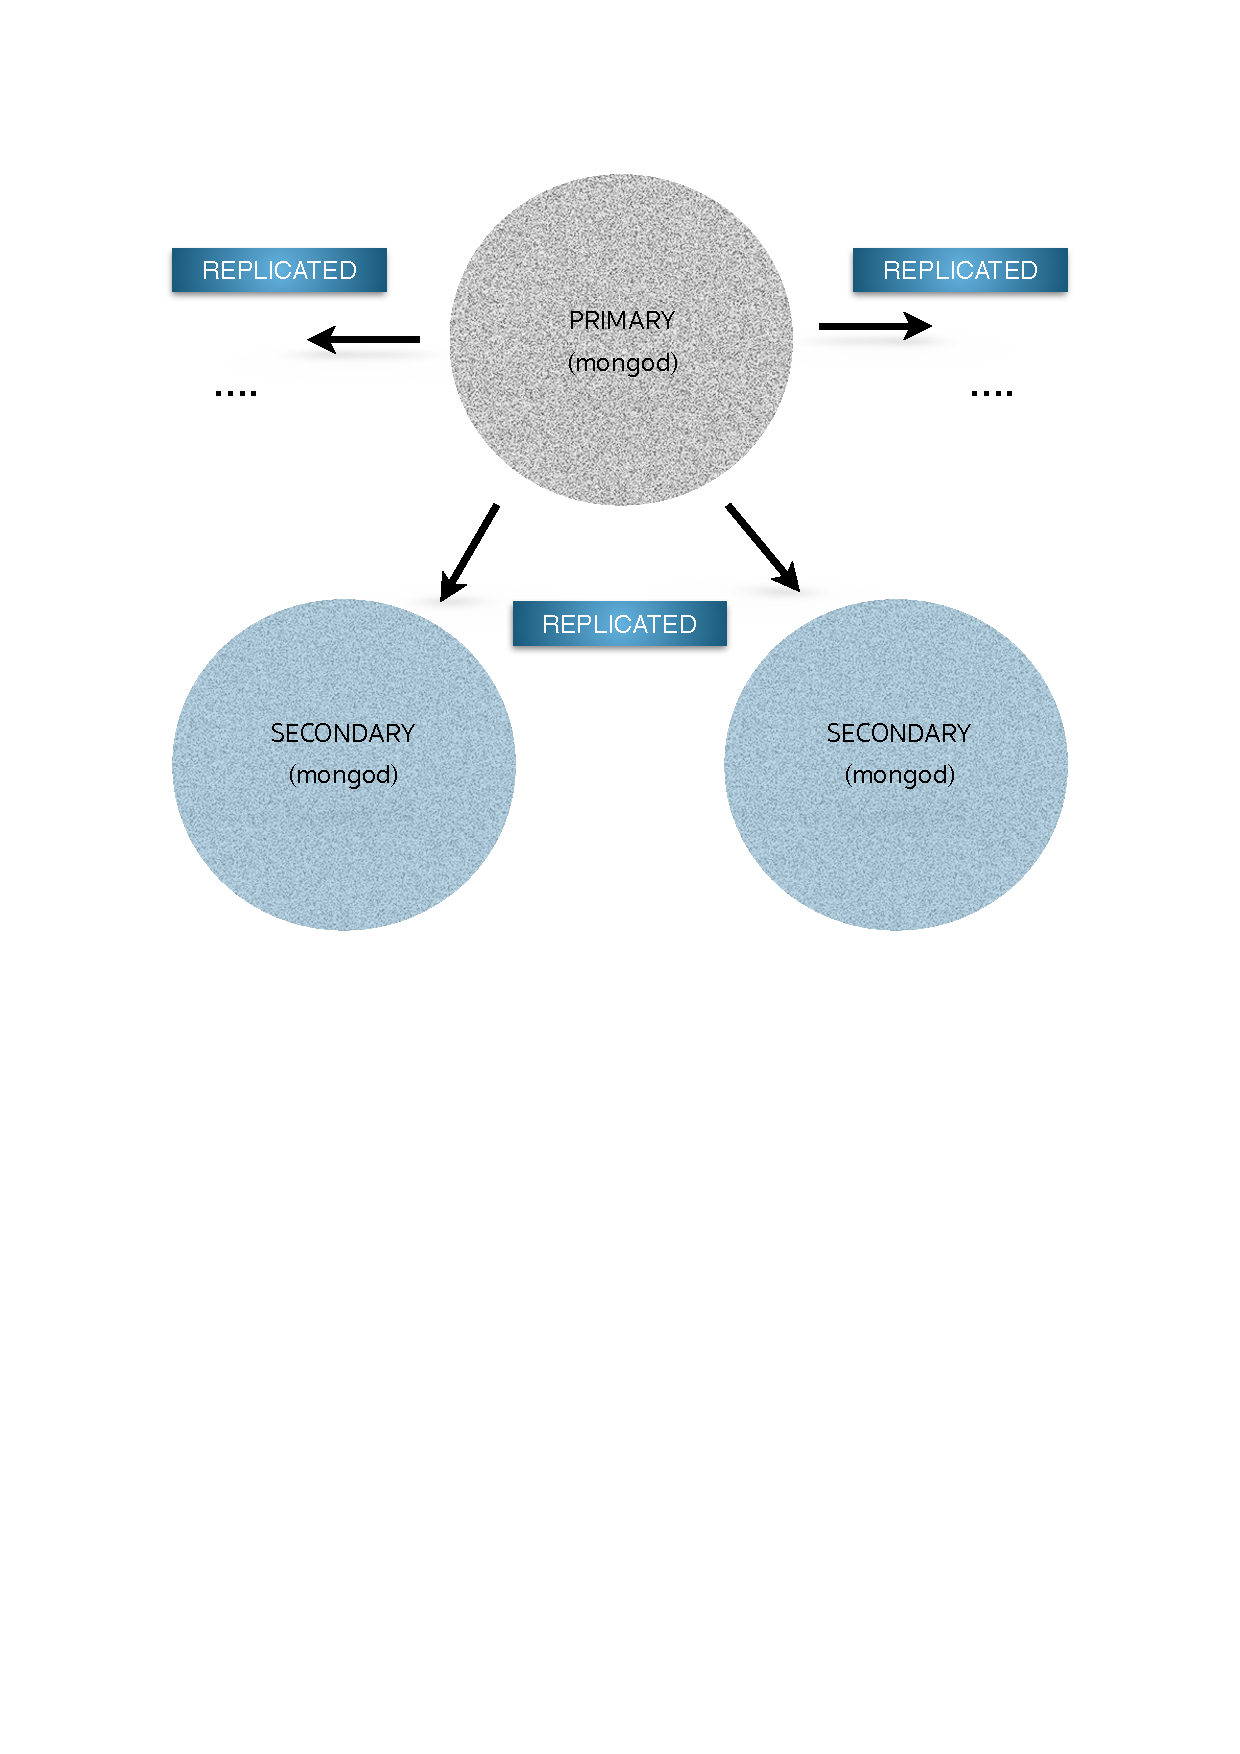
\includegraphics[trim = 20mm 0mm 28mm 24mm, clip, width=0.6\textwidth]{img/replicaSet}
\end{center}
\end{frame}

\begin{frame}
\frametitle{Szenario für eine Replikationsgruppe mit drei Servern in einer Shard}
\begin{center}
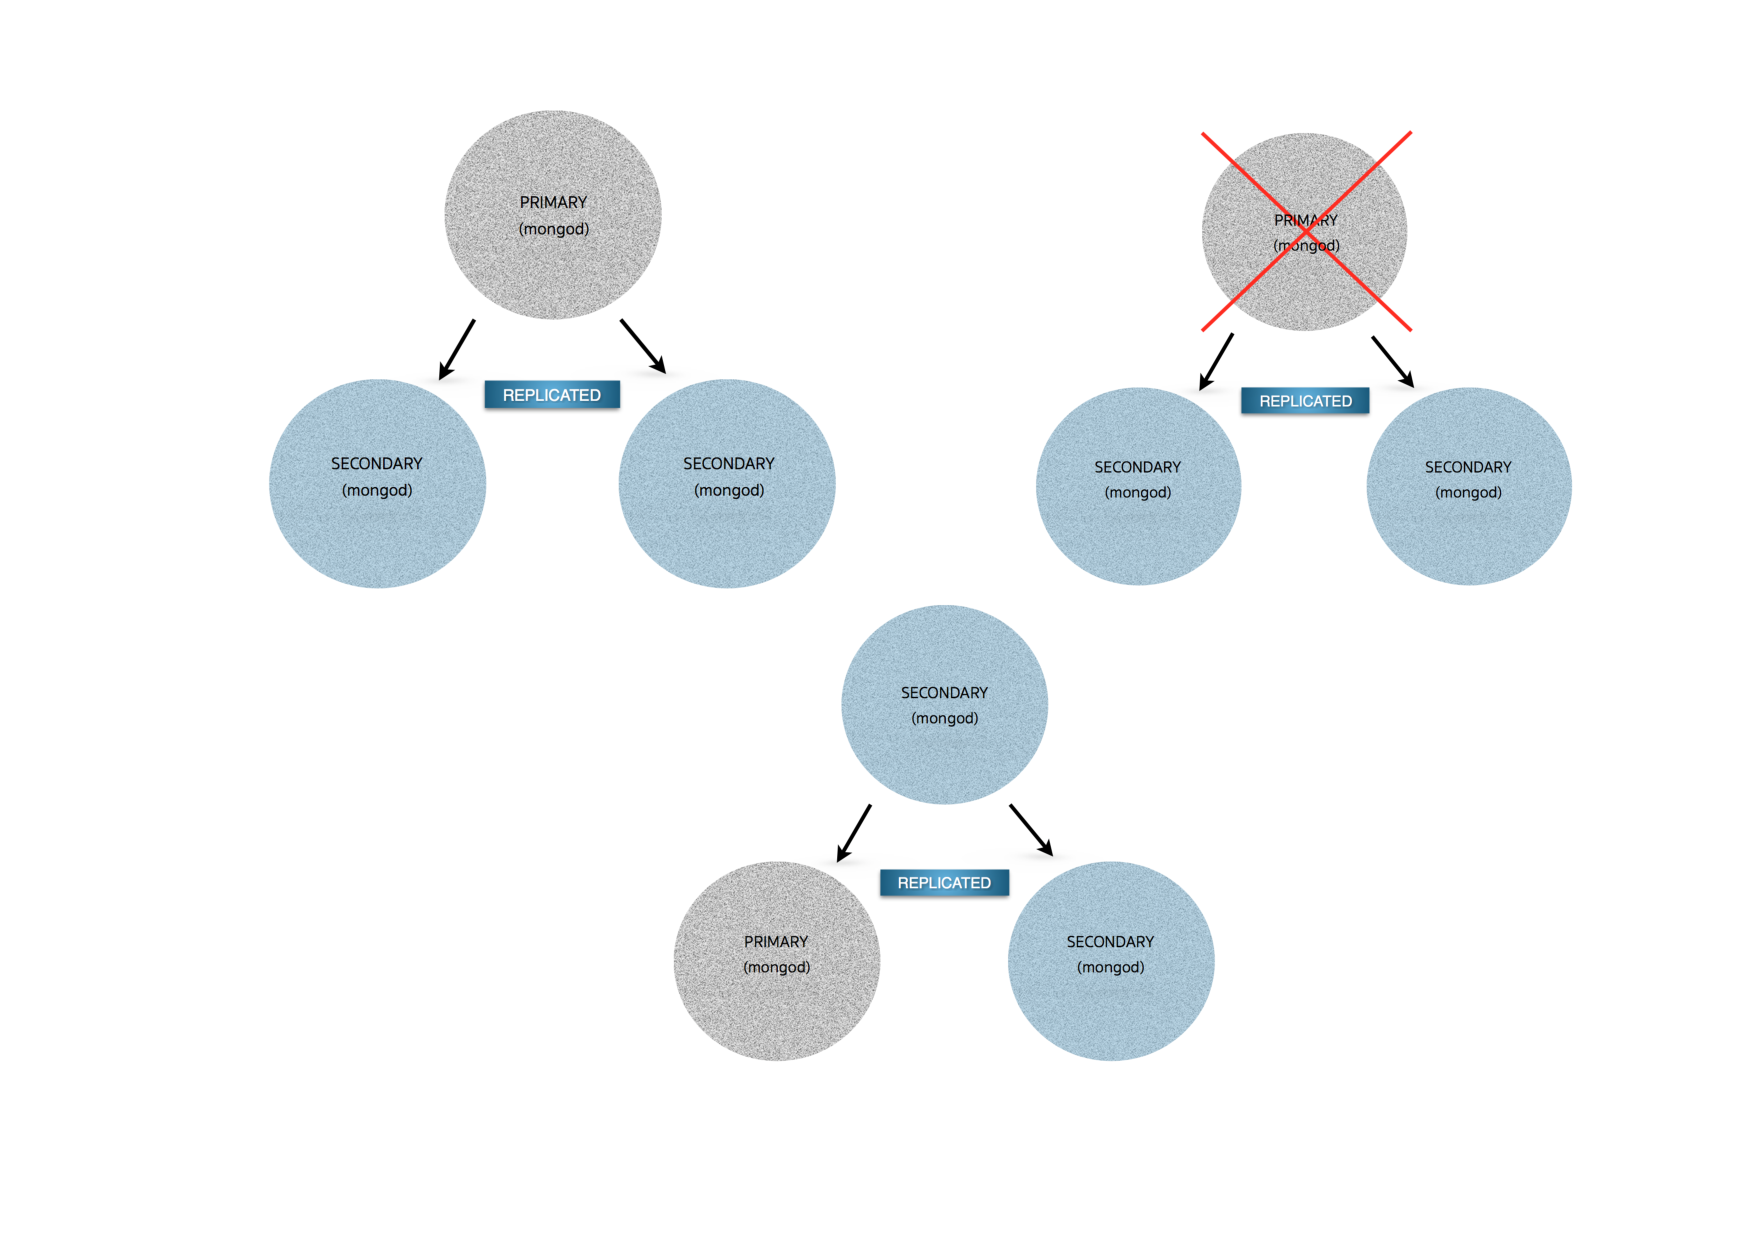
\includegraphics[trim = 0mm 0mm 0mm 5mm, clip, width=0.6\textwidth]{img/szenario}
\end{center}


\end{frame}

\begin{frame}
\frametitle{Freischaltung der Lesezugriffe}
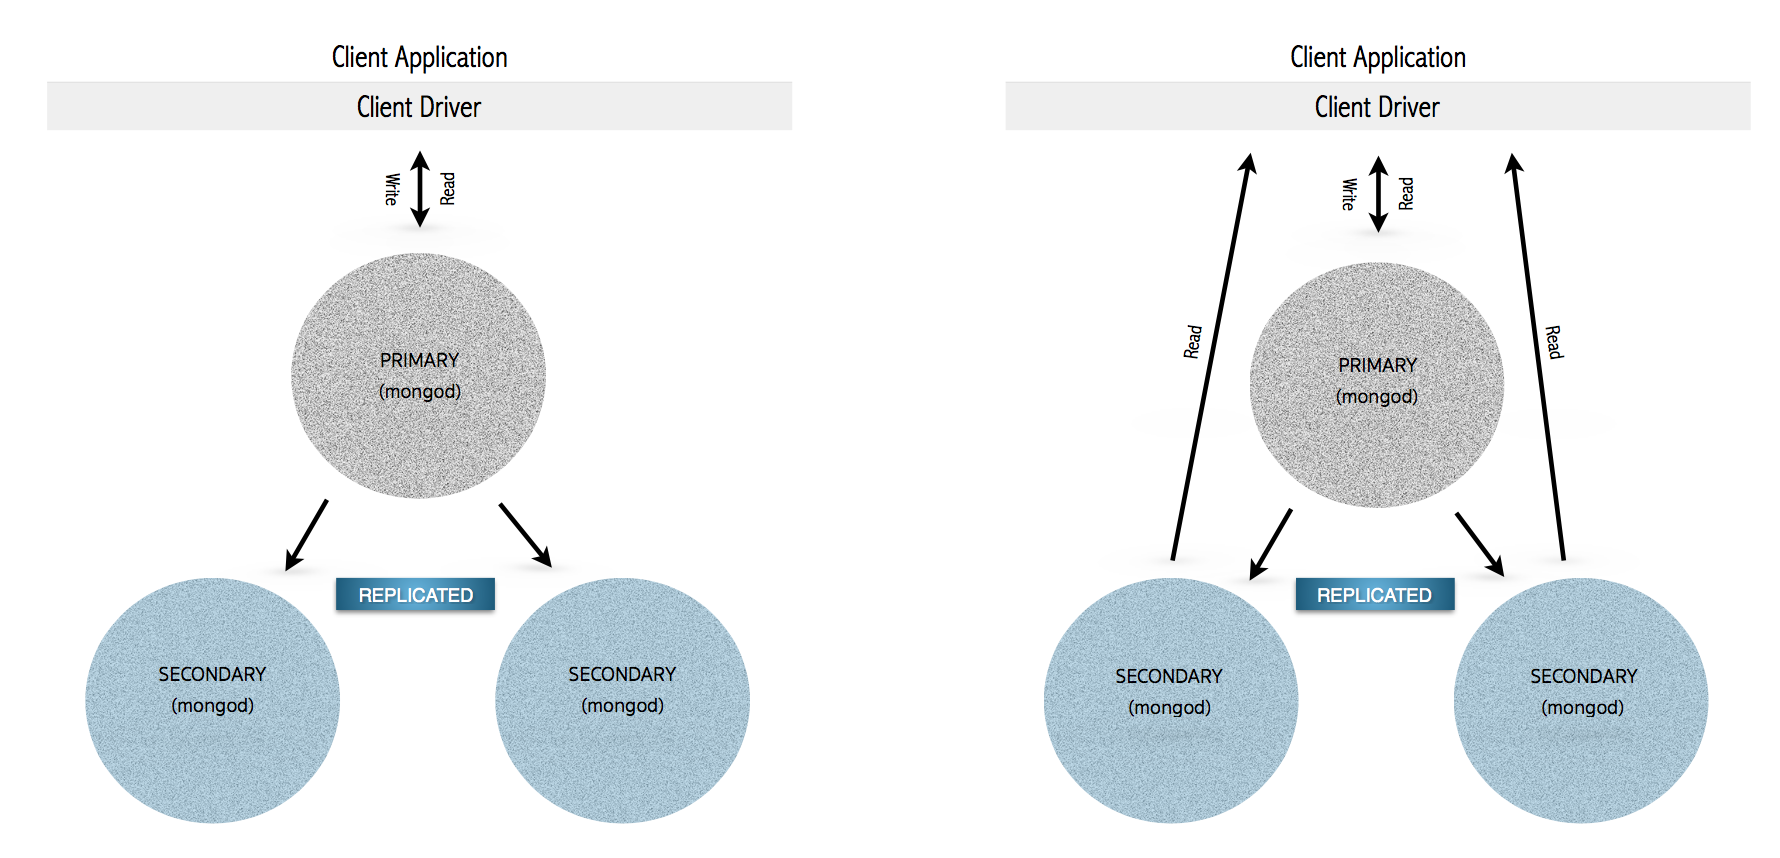
\includegraphics[width=1.0\textwidth]{img/slaveOK}
\end{frame}

\begin{frame}
\frametitle{MongoDB: Horizontale Skalierung (Sharding)}
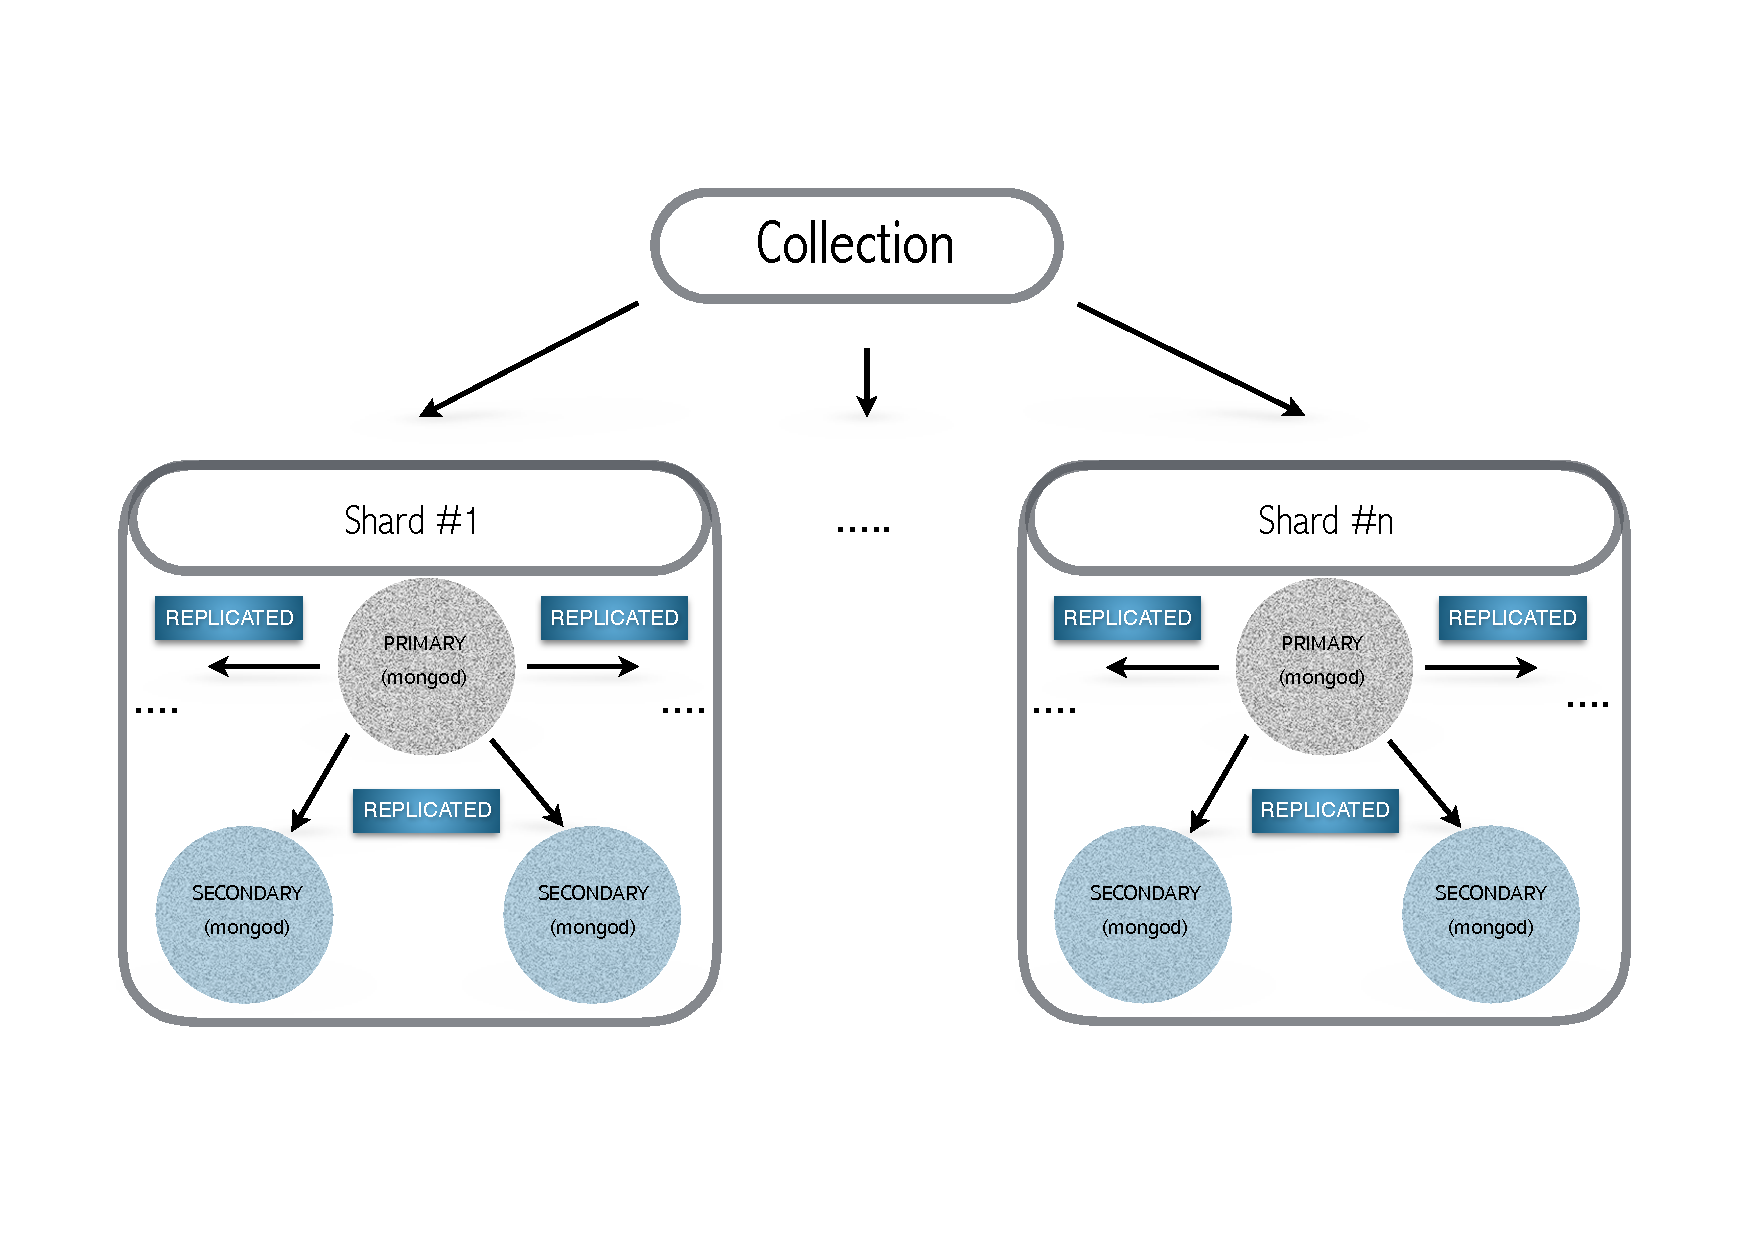
\includegraphics[trim = 0mm 35mm 0mm 30mm, clip, width=1.0\textwidth]{img/sharding}
\end{frame}

\begin{frame}
\frametitle{MongoDB: Sharded Cluster}
\begin{center}
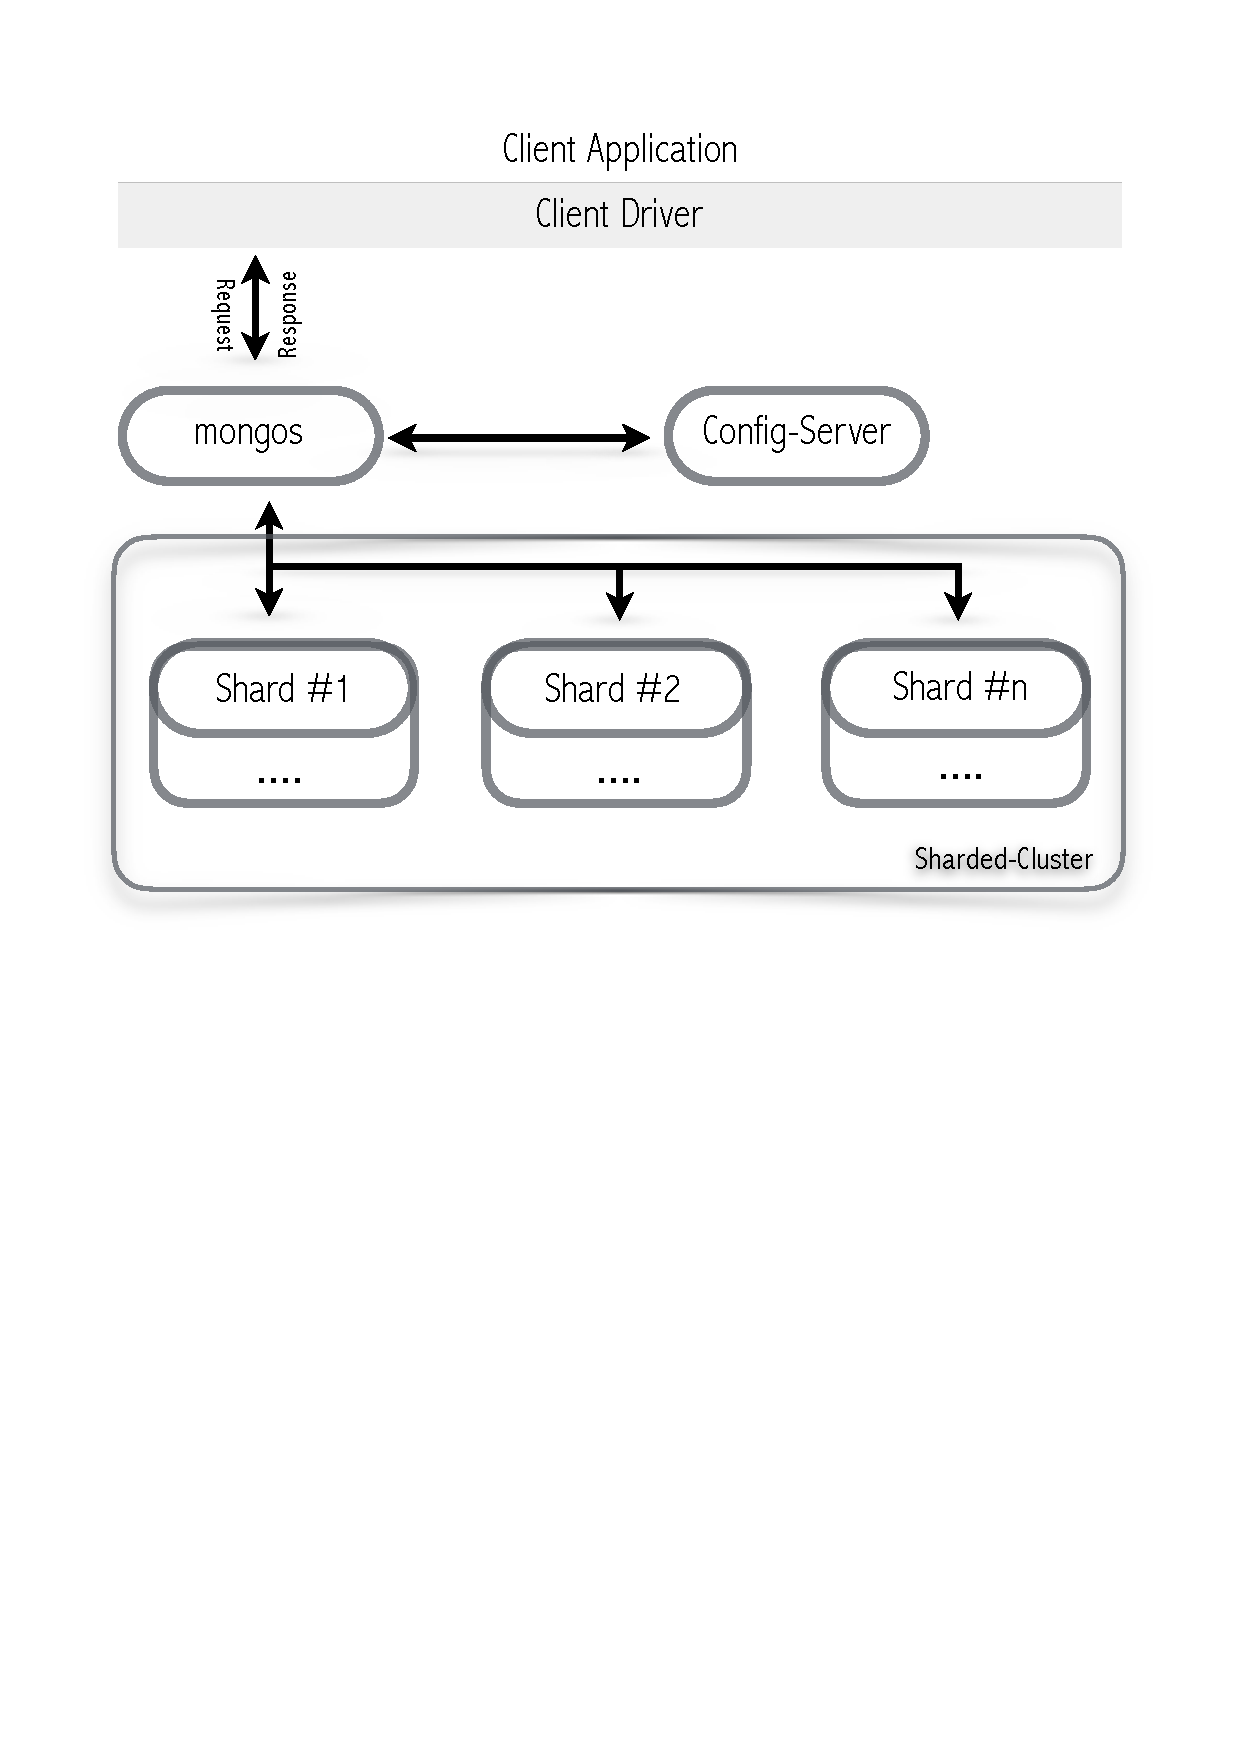
\includegraphics[trim = 0mm 139mm 0mm 22mm, clip, width=0.7\textwidth]{img/shardedCluster}
\end{center}
\end{frame}

\begin{frame}
\frametitle{Spring Framework (1)}
\begin{itemize}
\item Open Source Java Framework\newline
\item fundamentale Mission:
\begin{itemize}
\item die Entwicklung mit Java/Java EE zu vereinfachen\newline
\end{itemize}
\item zwei wichtige Kernstrategien:
\begin{itemize}
\item lose Kopplung durch „Injizieren“ von Abhängigkeiten und Interface-Orientierung

\item Reduzierung von Boilerplate-Code durch Vorlagen
\end{itemize}
\end{itemize}
\end{frame}


\begin{frame}
\frametitle{Spring Framework (2)}
\begin{itemize}
\item Verwaltung von einfachen Java Objekten, sogenannte Plain-Old-Java-Objects (POJO) durch Spring Framework als \textbf{Spring-Beans}.
\begin{center}
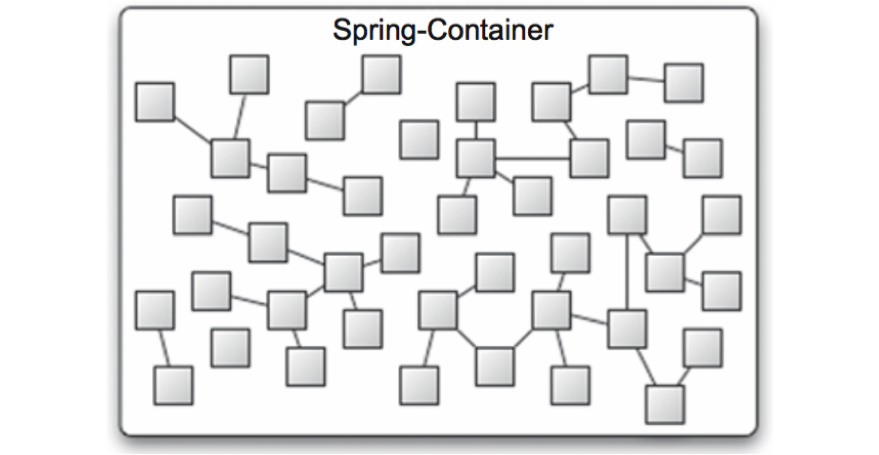
\includegraphics[width=0.5\textwidth]{img/container}
\end{center}
\item Spring nutzt POJOs bzw. Java-Beans, indem sie per DI zusammengesetzt werden.
\end{itemize}
\end{frame}

%\begin{frame}
%\frametitle{REpresentational State Transfer (REST)}
%
%REST ist ein Designkonzept für Web Services. Die Daten werden in der Form von Ressourceneinheiten ausgetauscht. Jede Ressource ist eindeutig und mit einer URI identifizierbar.\newline
%\begin{itemize}
%\item GET - ist ein lesender Zugriff auf Daten.
%\item PUT - aktualisiert bestehende Daten.
%\item DELETE - löscht vorhandene Daten.
%\item POST - legt neue Daten an.\newline
%\end{itemize}
%Die Rückmeldung des Web-Servers erfolgt im JSON-Format.
%\end{frame}


\begin{frame}
\frametitle{AngularJS 2 - JavaScript Framework}

AngularJS dient zur Entwicklung von so genannten Single-page-Anwendungen.\newline

In einer Single-page Webanwendung werden die HTML-Seite mit dem ganzen Inhalt nur einmal geladen und die Teile davon dynamisch nachgeladen oder upgedated.\newline

Entwickelt in TypeScript.
\end{frame}


%\subsubsection{Spring Framework}
%\begin{frame}
%\frametitle{Spring}
%bla
%\end{frame}
%
%\subsubsection{REST}
%\begin{frame}
%\frametitle{REST}
%bla
%\end{frame}
%
%\subsubsection{AngularJS 2}
%\begin{frame}
%\frametitle{AngularJS 2}
%bla
%\end{frame}


%\subsection[Architektur]{Umsetzbarkeit}
%\begin{frame}
%\frametitle{Umsetzbarkeit}
%bla
%\end{frame}




\section[Prototyp ive]{Prototyp live}
\begin{frame}
\begin{center}
\Huge !!! Live !!!
%\animategraphics[width=0.4\textwidth, controls]{1}{img/something-}{0}{9}
\end{center}

\includegraphics[width=0.5\textwidth]{img/smile-01}
\end{frame}





%\section[Fazit]{Fazit}
%\begin{frame}
%\frametitle{Fazit}
%\begin{itemize}
%\item Horizontale Skalierung - die bessere Wahl für verteilte Systeme
%\item \textit{stateless}- zustandslose Client-Anfragen ermöglichen n-Anzahl von Backends, die die Anfragen unabhängig voneinander parallel und effizient bearbeiten
%\end{itemize}
%\end{frame}


\begin{frame}
\begin{center}

\includegraphics[width=0.8\textwidth]{img/question}
\end{center}

\end{frame}



%\begin{columns}
%\column{0.6\textwidth}
%hola\pause

%\column{0.4\textwidth}
%\begin{itemize}
%\item test
%\item test
%\end{itemize}

%\end{columns}
%\only<1>{first}\only<2>{second}

%\end{frame}
\end{document}